\section[Appendix]{Appendix}
\label{fac:appendix}
\subsection{Bug Correction in synfast 2.14}
\label{fac:sec:bug_synder}
Thanks to the routine {\tt alm2map\_der}, the Fortran90 
\htmlref{{\tt synfast}}{fac:synfast} 
facility  produces
maps of $I,Q,U$ Stokes parameters and their first and second spatial derivatives,
starting from $C(l)$ or $a_{lm}$ coefficients.
{\bf A bug affecting the calculation of $\partial X/\partial\theta$, 
$\partial^2 X/\partial \theta^2$, 
$\partial^2 X/(\partial\theta\partial\varphi\sin(\theta))$, for $X=(Q,U)$
was detected in this routine and has been fixed in release 2.14 (March 2010).}

In what follows, the impact of this bug on the power spectra of
the produced maps is quantified, so that users can
assess how much their work could have been affected by this bug.

%-----------------------------------------------------
\begin{figure}[hb]
\latexhtml{%for latex
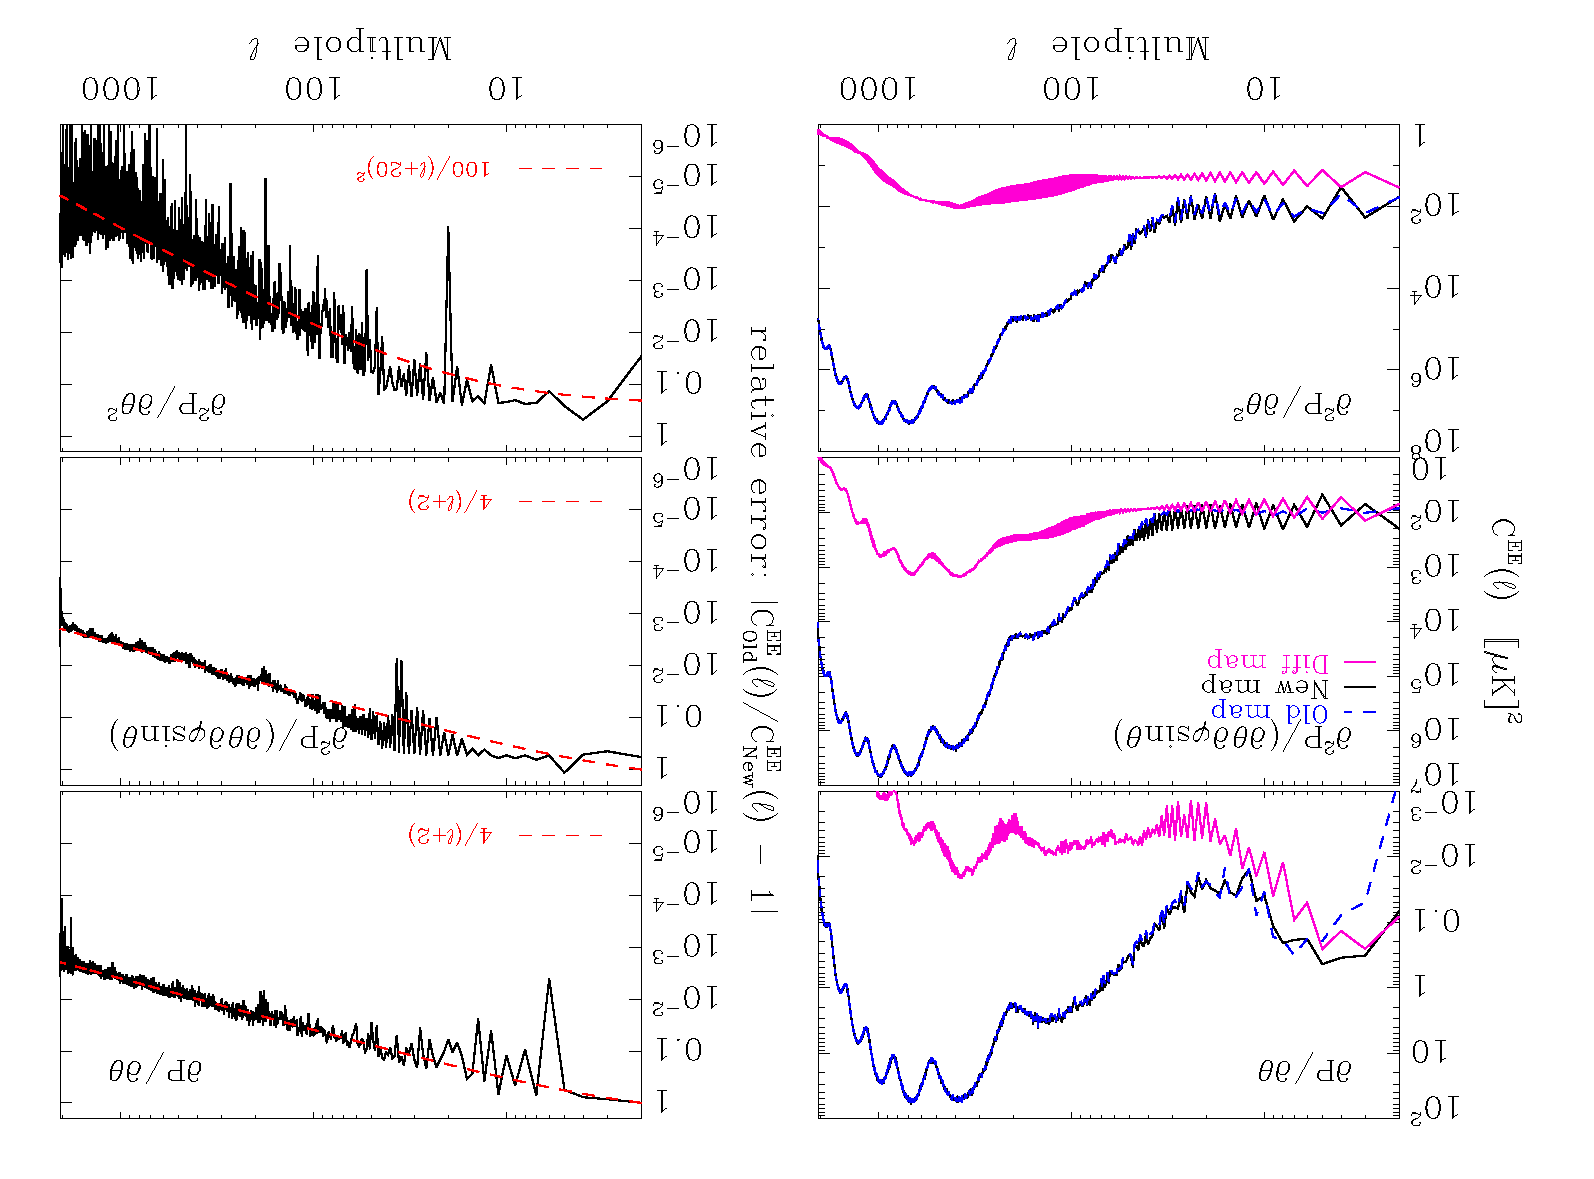
\includegraphics[width=0.99\textwidth,angle=-180]{fig/error_der.pdf}
}{%for html
\centerline{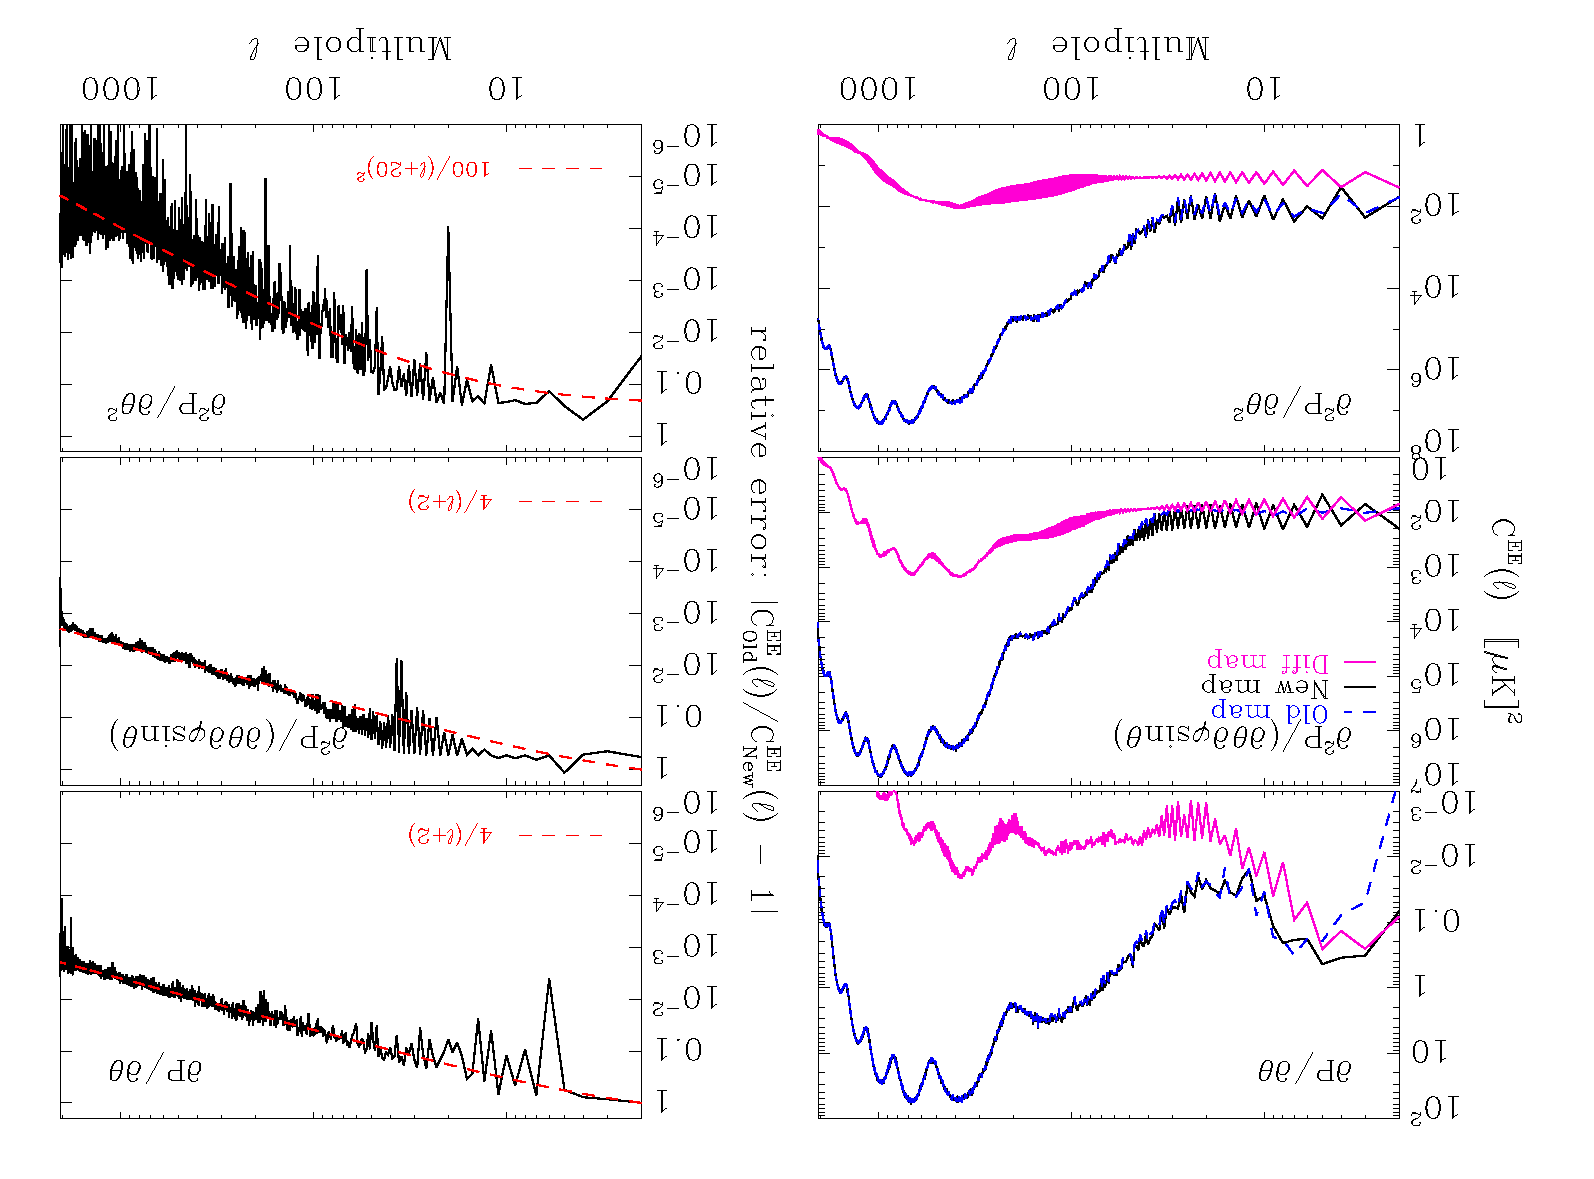
\includegraphics[width=520pt,angle=-180]{fig/error_der}}
}
\caption[Derivatives power spectra]{%
\label{fig:bug_derQU}\latexhtml{\footnotesize}{}%
Left panels: comparison of the EE power spectra $C(l)$ computed on polarized maps
derivatives generated by
{\tt synfast}-2.13a (Old maps, blue bashes), the bug corrected {\tt synfast}-2.14 (New maps, black lines)
and their differences (Diff maps, magenta lines). Note that what is plotted is
$C(l)$, {\em not} the customary $l(l+1)C(l)/2\pi$. Right panels show respectively
the relative error on the EE power spectrum of the old derivatives maps compared
to that of the new maps.
The red dashes show analytical fit to these errors.
}
\end{figure}
%-----------------------------------------------------
In Figure~\ref{fig:bug_derQU} we show the polarization $EE$ power spectrum of
$N_{\rm side} = 1024$ maps
in which the Stokes parameters $(Q,U)$ have been replaced by, in turn, their derivatives
$\partial (Q,U)/\partial\theta$, 
$\partial^2 (Q,U)/\partial \theta^2$, 
$\partial^2 (Q,U)/(\partial\theta\partial\varphi\sin\theta)$, 
for maps generated
by either the version 2.13a of {\tt synfast} or the corrected version 2.14, or
the difference of the two set of maps.
The input power spectra were those of WMAP-1yr $\Lambda$-CDM best fit model with a Gaussian
beam FWHM of 10 arcmin. The power spectra were computed on the whole maps, except
for 12 pixels around each pole that were masked out, because they get very
bright in second order derivatives.

It can be seen that the relative effect of the computation error on the produced maps was
large at low $\ell$, at scales on which derivatives maps contain little power, but decreasing
steadily with $\ell$.


\vskip 1cm
It should be stressed that the following quantities were {\em not} affected by
the bug described above:
\begin{itemize}
\item the Stokes parameters themselves $(I,Q,U)$,
\item the intensity $I$ and all its derivatives,
\item the Laplacians $\Delta I, \Delta Q$ and $\Delta U$, with
$\Delta \equiv \left(
\frac{\partial^2}{\partial\theta^2}
+ \cot\theta\frac{\partial}{\partial\theta} + 
\frac{\partial^2}{\sin^2\theta\partial\varphi^2} 
\right)$.
\end{itemize}
